\documentclass[a4paper]{report}
\usepackage{refstyle}
\usepackage{float}
\usepackage{booktabs}

\usepackage{Sweave}
\begin{document}
\Sconcordance{concordance:myfile.tex:myfile.Rnw:%
1 5 1 1 0 14 1 1 2 1 0 2 1 9 0 1 2 7 1 2 2 8 1}



\title{Sweave Example 1}
\author{Mike Ooko}
\date(\today)

\section{Introduction}
This is what we are moving to


\maketitle
In this example we embed parts of the examples from the
\texttt{kruskal.test} help page into a \LaTeX{} document:
\begin{Schunk}
\begin{Sinput}
> data(airquality)
> library(epicalc)
> kruskal.test(Ozone ~ Month, data = airquality)
\end{Sinput}
\begin{Soutput}
	Kruskal-Wallis rank sum test

data:  Ozone by Month
Kruskal-Wallis chi-squared = 29.2666, df = 4, p-value = 6.901e-06
\end{Soutput}
\end{Schunk}
which shows that the location parameter of the Ozone
distribution varies significantly from month to month. Finally we
include a boxplot of the data:


\begin{figure}[H]
\begin{center}

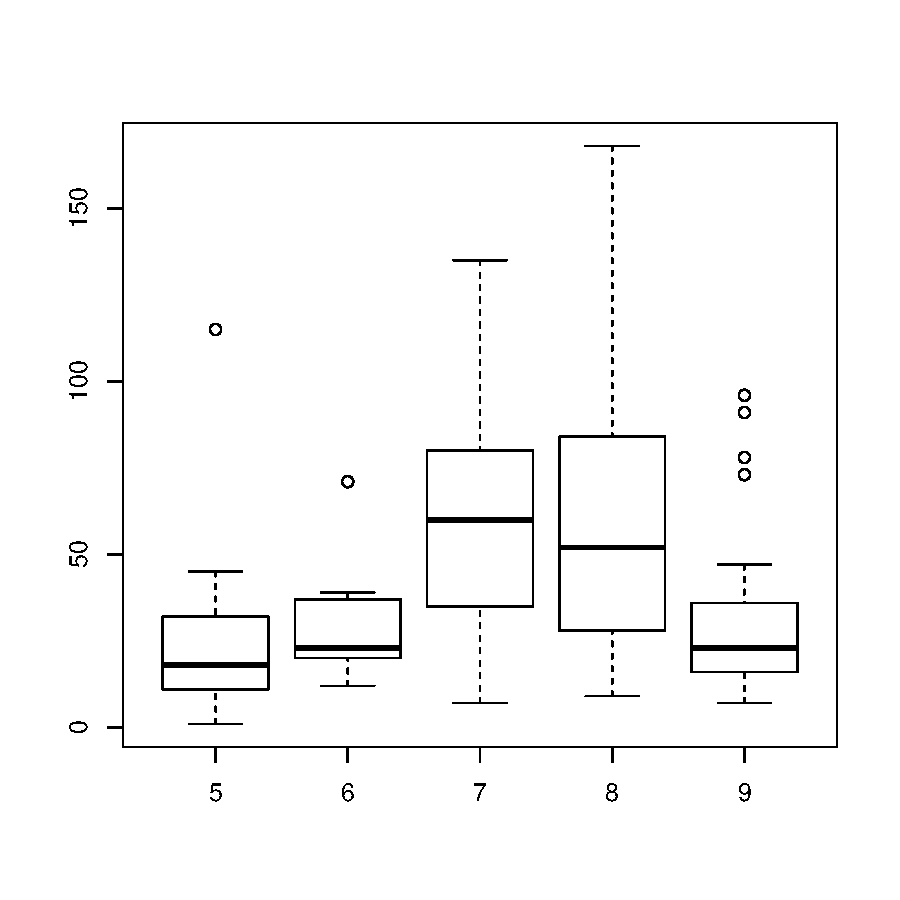
\includegraphics{myfile-002}

\end{center}
\caption{A boxplot of ozone by month}
\label{fig:fig1}
\end{figure}


The median zone is highest in August, as shown in \figref{fig1}.
\end{document}
